
\chapter{Nuclear Physics in Ultra-relativistic Heavy-Ion Collisions}

\section{The Standard Model}

The Standard Model describes the fundamental particles of the universe in terms of fermions and bosons. Fermions are particles with half-integer spin, while bosons have integer-spin. This difference in spin has far reaching consequences. Fermions must obey the Pauli Exclusion Principle: only one fermion at a time can occupy a given state. However, multiple bosons can simultaneously occupy a specific state.

Among the fermions are the leptons, neutrinos, and quarks. The leptons consist of the electron, muon, and tau, as well as their anti-particles. The leptons are seemingly fundamental: high energy experiments have yet to observe internal lepton-structure. Neutrinos are weakly interacting particles detected primarily through the precise measuring of missing transverse energy in the products of particle collisions. Quarks are the constituent particles of baryons, which contain three valence quarks, and mesons, which contain two valence quarks. In addition to the valence quarks are the sea quarks, which appear and disappear as quark-antiquark pairs within hadrons. The hadrons are particles made of quarks and gluons. See figure \ref{fig:halzen1p1} for the enumeration of elementary particle quantum numbers. 

\begin{figure}[h!]
\begin{centering}
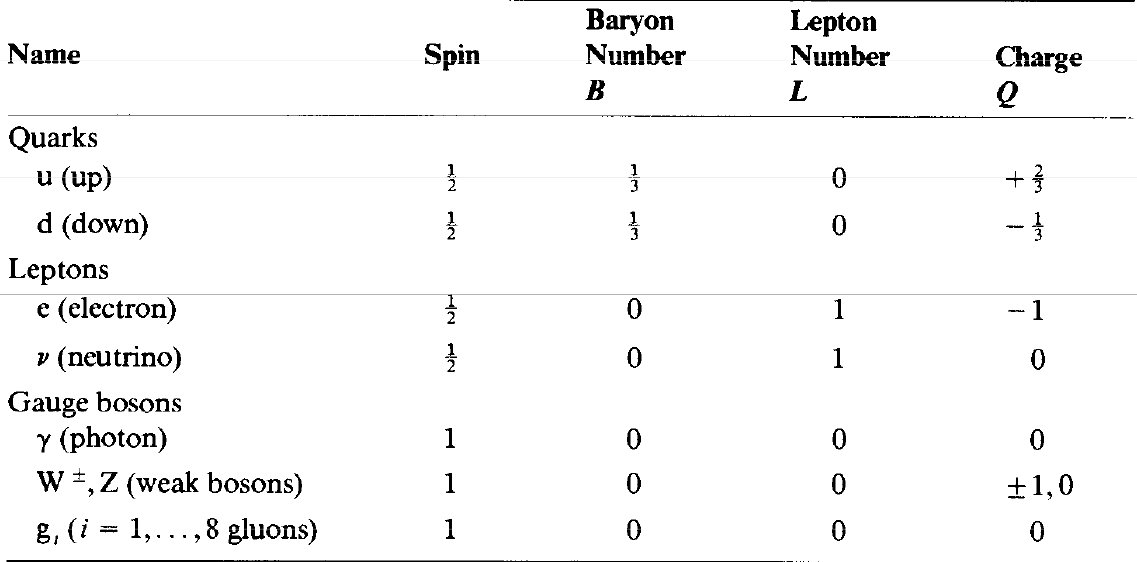
\includegraphics[width=6in]{Chapter1/importfigs/halzen_1_1.png}
\par\end{centering}
\caption{Elementary Particles and Quantum Numbers \label{fig:halzen1p1}}
\end{figure}

The behavior of fundamental particles is best described within the framework of quantum field theory (QTF). QFT defines a Lagrangian for fundamental particles. This Lagrangian then predicts the outcome of particle collisions. Different terms in the Lagrangian correspond to the various interactions between particles. The Standard Model Lagrangian, $\mathcal{L}_{Standard Model}$ can be broken down into three basic terms:

\begin{equation}
\mathcal{L}_{Standard Model} = \mathcal{L}_{QED} + \mathcal{L}_{QCD} + \mathcal{L}_{Higgs} + ... ,  
\end{equation}

Where $\mathcal{L}_{QED}$ is the QED Lagrangin, $\mathcal{L}_{QCD}$ is the QCD Lagrangian, and $\mathcal{L}_{Higgs}$ is the Higgs Lagrangian. The QED and QCD Lagrangians will be the most important in what follows. 

The most accessible approach to quantum field theory is through the use of Feynman diagrams. First, one imagines an interaction between particles. Then, one draws this process into a Feynman diagram, which is essentially a pictorial representation of exchanges between particles. The Lagrangian can be interpreted into Feynman rules. These rules describe how the Feynman diagram translates into a calcuation for the quantum mechanical amplitude of the process. The quantum mechanical amplitude, in turn, is proportional to the cross-section of the process. This is important because, sense the cross-section is invariant between experiments, one can use it to effectively test for invariant quantities in the Lagrangian.

\section{Quantum Electrodynamics}

Quantum electrodynamics (QED) is a theory of electromagnetic interaction in terms of relativistic quantum field theory. QED addresses three specific processes: photon motion, electron motion, and the emission, or absorption, of a photon by an electron. To do this, first a Lagrangian is established based on Maxwell's laws and quantum mechanics. The photon constitutes a spin-1 solution to Maxwell's equations. Likewise, electrons are described, at non-relativistic scales, by the Schrodinger equation, at relativistic scales by the Dirac equation. Figure \ref{fig:qedFeynman} shows the resulting processes allowed by QED: the translation of an electron, the translation of a photon, and the scattering of a photon off an electron.

\begin{figure}[h!]
\begin{centering}
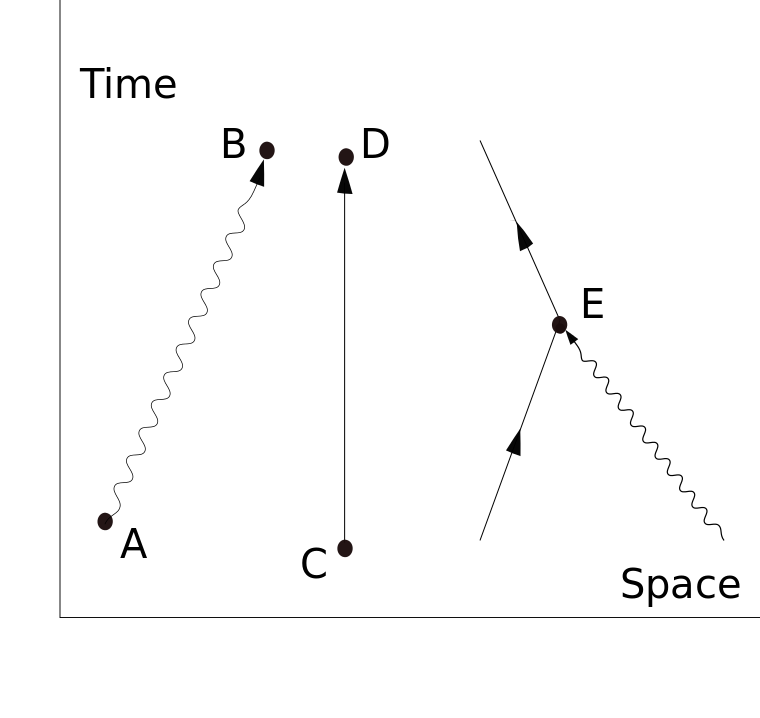
\includegraphics[width=4in]{Chapter1/importfigs/Feynman_Diagram_Components.png}
\par\end{centering}
\caption{QED Components of Feynman Diagrams \label{fig:qedFeynman}}
\end{figure}

The QED coupling constant is approximately ~1/137 at perturbative scales. However, at small scales, i.e. non-perturbative momentum transfers $Q^2$, the coupling constant increases.

\begin{equation}
\alpha_{QED}(Q^2) = \frac{ \alpha_{em}}{(1 - \frac{\alpha_{em}}{3\pi})\mathrm{ln}(\frac{Q^2}{m^2}) } ,
\end{equation}



\section{Quantum Chromodynamics}

The quarks are a family of fermions that compose the baryons and the mesons. Baryons consist of three quarks in a color neutral state, while mesons consist two quarks in a color neutral state. "Color" in this context refers to the six kinds of strongly-interacting charge available to quarks: red and anti-red, blue and anti-blue, and green and anti-green. Color charge has no relation to optical phenomena, but provides a useful analogy for the stable combinations of quarks. The net color-charge of a baryon or meson is "white".

Gluons are the QCD analogues of the photons in QED. Gluons are spin-1 and massless, but unlike photons, which do not carry electromagnetic charge, gluons carry strongly-interacting charge: color. Color comes six varieties: red, antired, blue, antiblue, green, and antigreen. 

Unlike QED, the QCD coupling increases with distance. Fig.\ref{fig:runningQCDCoupling} shows the running of the QCD coupling with $Q^2$. This has the practical consequence of the strong-interactions being stronger in high momentum transfer collisions. The direct results of the running QCD coupling are the dual phenomena of asymptotic freedom and color confinement. At large distances, string tension describes the binding force of the quarks. At short distances, however, Coulomb-like interactions dominate.

\begin{figure}[h!]
\begin{centering}
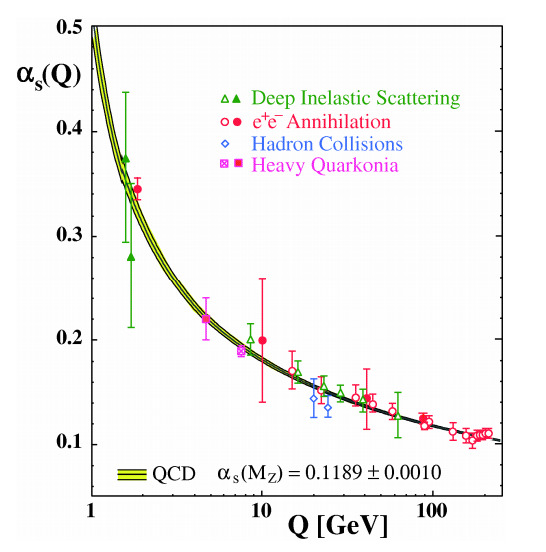
\includegraphics[width=4in]{Chapter1/importfigs/qcd_coupling_bethke.png}
\par\end{centering}
\caption{QCD Coupling Constant vs. $Q^2$ \label{fig:runningQCDCoupling}}
\end{figure}

Within the nucleus, a proton can be thought of as a bubble in a vacuum. Debrye screening exerts a pressure on the proton. This pressure is responsible for the size of the proton. 

\begin{equation}
\alpha_{QCD}(Q^2) = \alpha_{s}(Q^2) = \frac{4 \pi }{(11 - \frac{2}{3}n_f)\mathrm{ln}(\frac{Q^2}{\Lambda^2_{QCD}}) } ,
\end{equation}

\section{QCD Experiments}

Scattering experiments are the basic tool for exploring the nucleus. The Large Hadron Collider (LHC) is capable of reaching heavy-ion collision energies of up to 7 TeV per nucleon-nucleon. The higher the energy, the more experiments can probe the nuclear phase-space diagram. Momentum transferred, expressed as $Q^2$, is an important quantity for characterizing QCD measurements. In addition to $Q^2$, Bjorken-x, also known as Bjorken-scaling is necessary to describe the nuclear phase space. Bjorken-x represents the momentum fraction of partons. 

At the turn of the century, Ernst Rutherford probed the gold atom by bombarding a gold sheet with alpha-particles (helium nuclei). The angular distribution of the scattered alpha-particles demonstrates that the mass of the atom is concentrated in a small volume, i.e, the atom is mostly empty space. Further expedriments revealed that the atomic nuclei consisted of separate positively and neutrally charged particles: protons and neutrons. 

The modern understanding of subnuclear physics is based on results from three laboratories: Lawrence Berkeley National Laboratory (LBNL), Brookhaven National Laboratory (BNL), and CERN. Fixed target experiments hinted at the existence of a quark gluon plasma, but the collision energies were too low for this state to last. These experiments confirmed the developing model of the QCD phase space (Fig.\ref{fig:QCDPhase}).

\begin{figure}[h!]
\begin{centering}
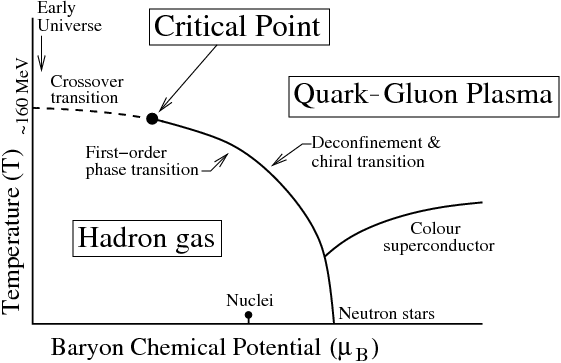
\includegraphics[width=4in]{Chapter1/importfigs/byr13.png}
\par\end{centering}
\caption{QCD Phase Diagram \label{fig:QCDPhase}}
\end{figure}

Collider experiments are capable of reaching much higher energies than fixed target experiments because of relativistic effects. 

\section{Deep Inelastic Scattering}

Deep inelastic scattering commonly refers to the scattering of a leptons off hadrons. Experiments at HERA focused on electron-proton collisions. In these collisions, the electron was used as a source of photons and neutrinos. When these particles scatter off the proton, the dependence of the collision cross section, on momentum transfer and scattering angle of the source electron, reflects the structure of the proton. These experiments provided the first evidence of two phenomena: the parton model and Bjorken-scaling. 

The parton model, first proposed by Richard Feynman, posits that hadrons in general, and nucleons in specific, are made of more fundamental constituent particles which may or may not be the quarks implied by the SU(3) symmetry. In addition to the quarks, the partons also include any field quanta associated with nuclear forces. In time, these field quanta are dubbed "gluons".

"Scaling" is an interpretation of the data from deep inelastic scattering (DIS). First proposed by James Bjorken, scaling is reflected in the incoherence of photon-proton interactions at photon energies above 1 $GeV/c$. Predictions from perturbative QCD are in good agreement with DIS data from HERA, as seen in .\ref{fig:qcdBjorkenX}.

\begin{figure}[h!]
\begin{centering}
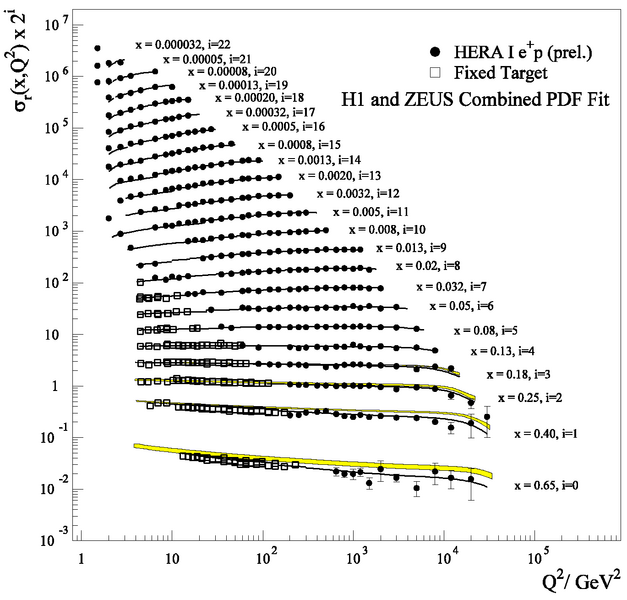
\includegraphics[width=4in]{Chapter1/importfigs/scholarpedia_bjorken_x_qcdExp.png}
\par\end{centering}
\caption{Collision Cross Section vs Bjorken-x, theory and data \label{fig:qcdBjorkenX}}
\end{figure}

Soft processes compose the low momentum transfer, typically gluon-gluon interactions during a  collision.

\section{Ultra-peripheral Heavy-Ion Collisions}

Similar to the Rutherford experiment, in heavy-ion collisions the scattered particles carry information about the internal structure of the nucleus. 

The Rutherford experiment has the three components that still characterize high-energy nuclear experiments: a probe, a medium, and a signal. Alpha particles probe the medium of the gold atom, and the angular distribution of scattered alpha particles signals the internal structure of the atom. 

Ultra-peripheral collisions occur at impact parameters greater than the sum of the heavy-ion radii. In these collisions, hadronic interactions are strongly suppressed while photonuclear activity is enhanced proportional to the square of the nuclear charge. The electromagnetic field of an incoming heavy-ion, from the perspective of a target, is equivalent to a flux of virtual photons; fig.\ref{fig:smushedField} illustrates the Lorentz contraction of the field of a boosted charge.

\begin{figure}[h!]
\begin{centering}
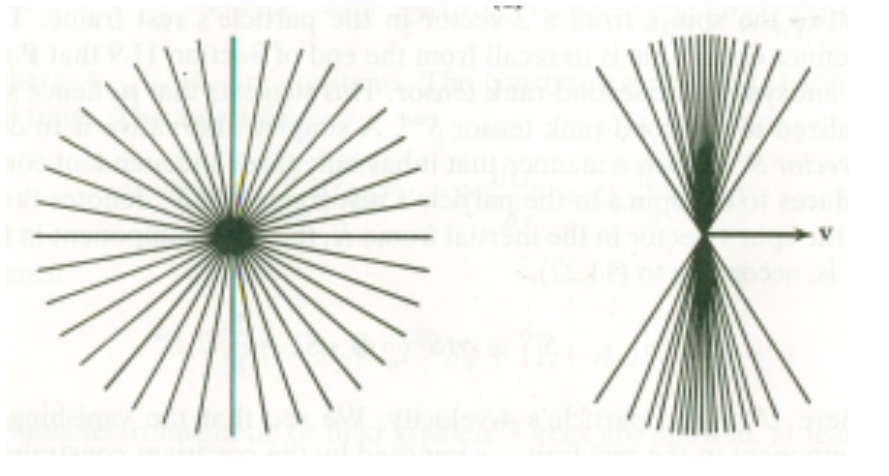
\includegraphics[width=4in]{Chapter1/importfigs/jackson_em_wwa.png}
\par\end{centering}
\caption{ (a.) electromagnetic field of stationary charge (b.) eletromagnetic field of boosted charge \label{fig:smushedField}}
\end{figure}

The Weizsacker-Williams appoximation (WWA) calculates the density of photons, about the nucleus, as a function of energy. WWA is a semi-classical formulation. Maxwell's equations are solved for a stationary point charge boosted to an ultra-relativistic velocity. In the target's frame, the Fourier transform of the source field is taken. The Fourier frequency modes are interpreted through the quantum mechanical equation of photon energy. The photon flux as function of energy is given by

\begin{equation}
N(\omega,b) = \frac{\alpha}{\hbar \omega}\left( \frac{Z}{b\beta\pi} \right)^2\left ( \frac{\omega b}{\gamma \nu} \right )K_1^2\left ( \frac{\omega b}{\gamma \nu} \right ) ,
\end{equation}

where $K_1^2$ is a Bessel function.

Gluons are the particle exchanged in strong interactions. However, gluons themselves carry color charge. By analogy, photons transmit the electromagnetic force, but do not themselves have an electric charge. 

When a quark is scattered from a nucleus, the strong interaction gathers potential energy until the threshold for quark production is passed, at which point an anti-quark is generated to screen the ejected quark.

QCD factorisation describes the diffractive-photoproduction dijet cross-section as the convolution of the partonic cross-section with the diffractive parton distributions. However, factorisation only describes H1 data if the resolved-photon contribution is suppressed. 

The photoproduction cross-section is proportional to the gluon distribution. At low momentum transfer, photons interact electromagnetically, i.e. directly, with partons. High energy, "resolved" photons possess a hadronic structure; instead of directly interacting with the nuclei, these photons fluctuate into mediating quark-antiquark pairs. 

\section{Factorization}

Diffractive dijet photoproduction is not describable in perturbative QCD. For coherent processes the photon energy is small, and therefore the wavelength is large compared to the size of the nucleus. At these large distances, there isn't a hard scale, and so perturbation calculations cannot be done. Gluon splitting interactions dominate the low Bjorken-x partons. QCD collinear factorization describes these soft interactions via the convolution of parton cross sections, taken from perturbative QCD, and diffractive parton distribution functions, taken from experiment. 

\begin{figure}[h!]
\begin{centering}
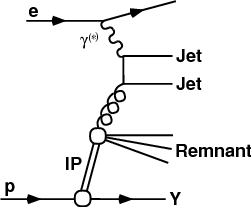
\includegraphics[width=2.2in]{Chapter2/importfigs/fig1a.png}
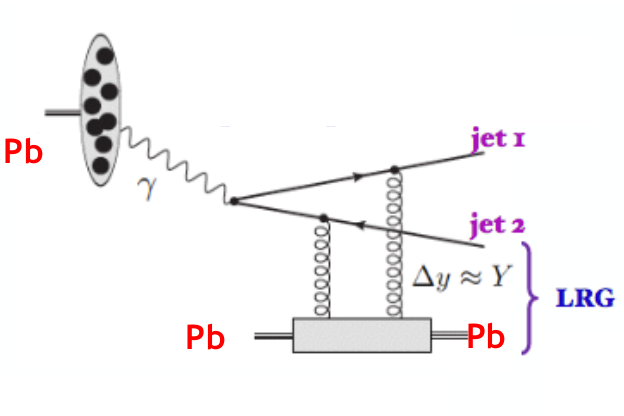
\includegraphics[width=3in]{Chapter2/importfigs/fig3_daniel_upc.png}
\par\end{centering}
\caption{Feynman diagrams for coherent jet photoproduction in (a.) lepton-proton collisions and (b.) Pb-Pb collisions \label{fig:feynmanUPC1}}
\end{figure}

In electron-hadron collisions, diffractive photoproduction is characterized by the presence of a large rapidity gap in the final state and an intact nucleus. The Feynman diagram of electroproduction in lepton-hadron collisions is similar to that of photoproduction in ultraperipheral collisions, as seen in fig.\ref{fig:feynmanUPC1}. The diffractive dijet cross section is expressed by the convolution of partonic cross sections $d\hat{\sigma}$ and diffractive PDFs $f^D_{i/p}$.

\begin{equation}
d\sigma (ep \rightarrow e + 2 jets + X^{'} + p) = \sum_{i} \int dt \int dx_\mathbb{P} \int dz_\mathbb{P} d\hat{\sigma}_{ei\rightarrow 2jets}(\hat{s},\mu^2_R,\mu^2_F)\times f^D_{i/p}(z_\mathbb{P},\mu^2_F,x_\mathbb{P},t) ,
\end{equation}

In the proton-vertex factorisation hypothesis, the dependence on $x_{\mathbb{P}}$ and $|t|$ is factored out of the dependence on $\mu^2_F$ and $z_{\mathbb{P}}$. Furthermore, $f^D_{i/p}$ is sum of contributions from the Pomeron and Reggeon:

\begin{equation}
f^D_{i/p}(z_{\mathbb{P}},\mu^2_F,x_{\mathbb{P}},t) = f_{\mathbb{P}/p}(x_{\mathbb{P}},t)f_{i/\mathbb{P}}(z_{\mathbb{P}},\mu^2_F) + n_\mathbb{R}f_{\mathbb{R}/p}(x_{\mathbb{P}},t)f_{i/\mathbb{R}}(z_{\mathbb{P}},
\mu^2_F) ,
\end{equation}

Lepton-hadron collisions were performed at HERA and measured by the H1 experiment. These experiments reported a value for the total diffractive photoproduction cross section that is double that predicted by QCD collinear factorization; fig.\ref{fig:h1Ratio} compares the cross-section of H1 data to that predicted by NLO-QCD. Diffractive events were selected for using rapidity gaps or the presence of leading protons in the very forward proton spectrometer (VFPS). 

\begin{figure}[h!]
\begin{centering}
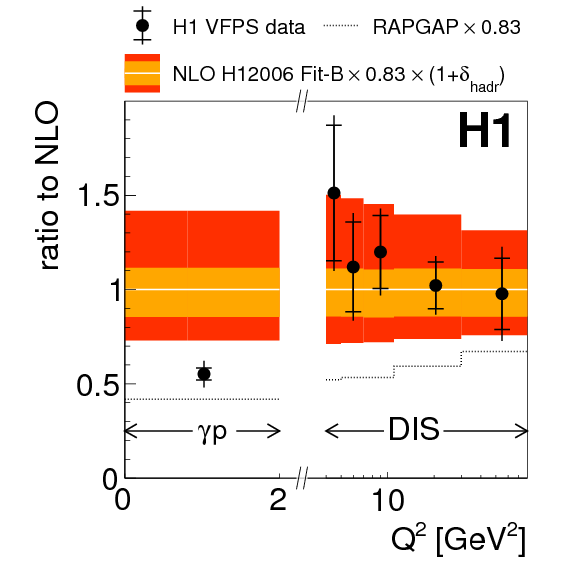
\includegraphics[width=3in]{Chapter2/importfigs/fig8_h1_2015.png}
\par\end{centering}
\caption{Ratio of H1 data cross-section to NLO-QCD cross-section \label{fig:h1Ratio}}
\end{figure}

H1 used the Very Forward Proton Spectrometer (VFPS) to trigger on low $Q^2$ protons. The VFPS consists of two Roman Pots located 218 m and 222 m from the H1 interaction-point in the forward direction. The VFPS can detect protons scattered at very low transverse momentum, corresponding to $0.008 < x_{P} < 0.028$ and $|t|<0.6$. Each of the Roman Pots contains layers of scintillating fibers, which are covered by a layer of scintillator tiles. The fibers readout to photomultipliers, and the tiles both shield from radiation and trigger on protons. The track effiency of VFPS is a remarkable $96 \%$, and the background contamination is kept at $1 \%$ , making the detector excellent for studying diffractive events. Fig.\ref{fig:h1BeamEnv} shows the $|t|$ coverage of the Forward Proton Spectrometer (FPS) and VFPS.

\begin{figure}[h!]
\begin{centering}
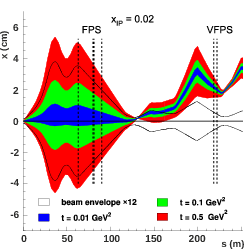
\includegraphics[width=3in]{Chapter2/importfigs/fig7_h1_2015.png}
\par\end{centering}
\caption{Beam envelope vs. distance to vertex in H1 \label{fig:h1BeamEnv}}
\end{figure}

The H1 data was compared to predictions based on NLO-QCD convoluted with diffractive parton distribution functions (DPDFs) from HERA inclusive diffractive deep-inelastic scattering (DDIS) data. For diffractive pp collisions the high transverse momentum jets yield a hard scale for perturbative QCD. 

\section{Wigner Distribution}

One can use the Wigner distribution to tomographically image the internal structure of the nucleus. The nucleus manifests different structures at varying momentum fractions; specifically, small momentum fractions exhibit gluon saturation (fig.\ref{fig:nuclImag}).

\begin{figure}[h!]
\begin{centering}
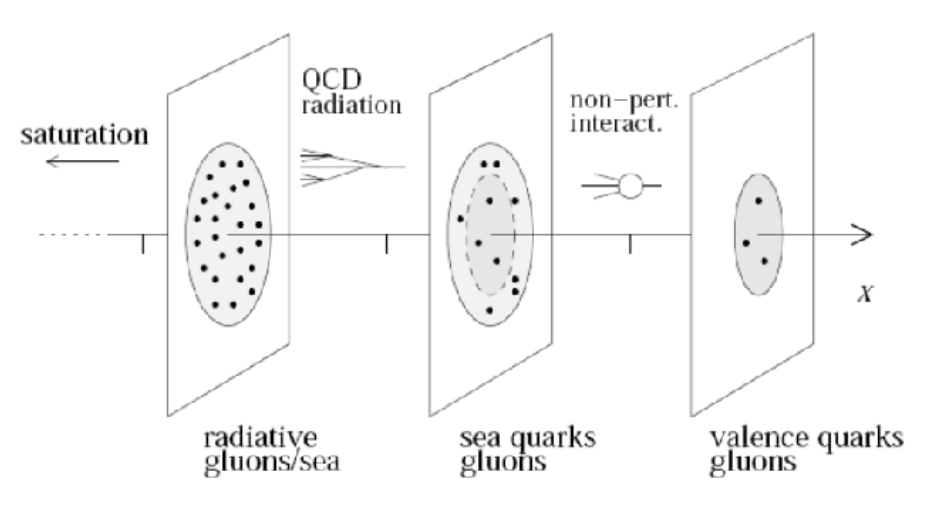
\includegraphics[width=7in]{Chapter2/importfigs/imaging_the_nucleon_upc_dijets_pres.png}
\par\end{centering}
\caption{Subnuclear tomography \label{fig:nuclImag}}
\end{figure}

The quantum field theory lagrangian of the strong interaction is relatively simple, but because of confinement and asymptotic freedom the hadronic bound states are too complex for an analytic solution. Furthermore, collider experiment data requires a quantitative interpretation to be useful. The gap between QCD and heavy-ion data is bridged using the parton model, which considers hadrons as composed of quarks and gluons. Parton density functions (PDFs) model the longitudinal momentum distribution of the partons. PDFs are supplemented by transverse momentum distributions (TMDs) and generalized parton distributions (GPDs). In addition to transverse momentum, GPDs describe the transverse spatial distribution. TMDs and GPDs are derived from the final state particles of a collision. Markus Diehl maps the relationship between various distribution functions in fig.\ref{fig:gpdTMDWeb}.

The Wigner distribution is a quantum phase space distribution that describes small-x gluons. Specifically, by considering the color diple scattering amplitude, the angular correlation of the nucleon recoil momentum and the dijet transverse momentum can provide a three-dimensional, tomographic image of the gluons within a high energy nucleus. This tomographic image takes the form of a Wigner distribution, which contains all the information of both TMDs and GPDs without violating the uncertainty principle. Specifically, the angular correlation directly measures the Fourier transform of the gluons. This is possible because the dipole amplitudes are functions of the impact parameter, and because collinear factorization holds. 

\begin{figure}[h!]
\begin{centering}
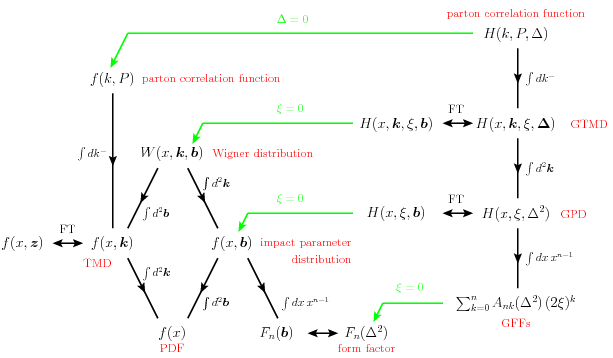
\includegraphics[width=7in]{Chapter2/importfigs/fig6_introGPD_TMD.png}
\par\end{centering}
\caption{Interconnectedness of Parton Distributions \label{fig:gpdTMDWeb}}
\end{figure}

TMDs and GPDs manifest non-perturbative QCD effects. The Wigner distribution, at this scale, reflects the relationship between the position and momentum of partons. Integrating the Wigner function over the transverse distance yields the TMD, while integrating over transverse momentum yields a GPD with spatial information. 

Yoshitaka Hatta uses the dipole framework to show that the azimuthal angular correlations of coherent dijets are generated by the underlying gluon Wigner distribution. Furthermore, these correlations are consistent with predictions based on standard collinear factorization. Relevant kinematic variables are mapped in the fig.\ref{fig:yatta1}.

\begin{figure}[h!]
\begin{centering}
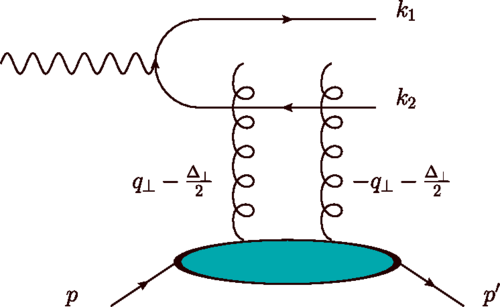
\includegraphics[width=4in]{Chapter2/importfigs/fig4_yatta.png}
\par\end{centering}
\caption{Feynman Diagram of Coherent Dijets in Dipole Framework. \label{fig:yatta1}}.
\end{figure}




